\documentclass[a4paper,twoside]{article}

\usepackage{epsfig}
\usepackage{subcaption}
\usepackage{calc}
\usepackage{amssymb}
\usepackage{amstext}
\usepackage{amsmath}
\usepackage{amsthm}
\usepackage{multicol}
\usepackage{pslatex}
\usepackage{apalike}
\usepackage{booktabs}
\usepackage{xcolor}
\usepackage{url}
\usepackage{algorithm2e}   % required by SCITEPRESS.sty
\usepackage[bottom]{footmisc}
\usepackage{SCITEPRESS}   % Add other packages BEFORE this line.

% ---- Draft helper: remove all \TODO before submission ----
\newcommand{\TODO}[1]{\textcolor{red}{\textbf{[TODO: #1]}}}

\begin{document}

% Working title — to be discussed with the team
\title{Decoupling Detection from Identification for Species-Level Fly Monitoring on Industrial Sticky Traps}

% DOUBLE-BLIND: keep anonymous until camera-ready (VISAPP requirement).
\author{\authorname{Anonymous Author(s)}
\affiliation{Anonymous Affiliation}
\email{anonymous@anonymous.org}
}

\keywords{Pest Monitoring, Sticky Traps, Tiny Object Detection, Fine-Grained Classification, Detection Cascade, Data-Centric AI.}

\abstract{Species-level monitoring of flies on industrial sticky traps combines tiny objects (mean box size $\approx$44\,px in 1920$\times$1080 images) with fine-grained distinctions between look-alike species. On DS-F2, a dataset extended with targeted physical collections, we test three levers with a YOLO26 detector. \emph{Data:} along five cumulative training sets, species accuracy rises from 56\% to 82\% (three seeds); random subsamples of the final set match the 244- and 869-image rungs, so there we detect no advantage of targeting over quantity, but the earliest lot is 19\,pp worse than a random subsample of its size. \emph{Identification:} with our recipe, a detect-then-classify cascade does not beat the detector in any of 15 configurations (nor with species-only relabelling, late fusion or other crop margins), and ground-truth-crop accuracy saturates near 83\% for five classifiers; ambiguous pixels, label noise and the crop recipe cannot be separated. \emph{Tiny-object methods} from aerial imagery (NWD, RFLA, P2 head, higher resolution, sliced inference) give no gain detectable with three seeds and default hyperparameters. All results come from one facility and a 73-image test split. Code will be released; the images will not.}

\onecolumn \maketitle \normalsize \setcounter{footnote}{0} \vfill

\section{\uppercase{Introduction}}
\label{sec:intro}

Flying insects are a major sanitary and economic threat in food-industry facilities, where regulatory compliance requires continuous monitoring of fly populations. Adhesive (sticky) traps are the standard monitoring instrument: cheap, passive, and ubiquitous. Their bottleneck is the manual inspection of each plate by technicians who must not only \emph{count} the insects but \emph{identify their species}, since different species imply different contamination sources. Automating this reading is therefore a species-level recognition problem, not merely a counting one.

Computationally, sticky-trap reading sits at the intersection of two regimes that are hard in isolation and rarely studied together. First, it is a \emph{tiny object} problem: in our industrial setting, plates are photographed at 1920$\times$1080 under a fixed-focus protocol, and the mean captured insect measures $\approx$44\,px ($\sqrt{wh}$), about 2\% of the image width, and a large share of the insects fall below the 32\,px limit commonly used to define ``tiny'' objects~\cite{cheng2023soda}; at native resolution, however, each insect still spans several feature-map cells. Second, it is a \emph{fine-grained} problem: the target species differ in subtle cues (wing venation, thorax patterning, size ratios) that degrade quickly as trapped specimens decay~\cite{bockmann2021}. Recent species-level work on sticky traps remains confined to laboratory conditions and single-stage detectors~\cite{laekeman2025}, while the tiny-object literature validates its methods almost exclusively on aerial imagery~\cite{wang2021nwd,xu2022rfla}, and detect-then-classify cascades for species identification are established for vertebrate camera traps~\cite{beery2019} but essentially untested on trap-caught insects.

Prior work introduced a data-centric pipeline for this exact setting~\cite{pacbb2026}: through iterative dataset curation, an explicit \emph{Noise} class and a fixed focal distance, a single-stage YOLO detector was driven from 0.476 to 0.608 mAP. That study concluded, however, that the remaining confusion between visually similar fly species was \emph{irreducible}: no further data curation reduced the misclassification between look-alike pairs. This claim frames the question we address here: \textbf{what limits species-level reading of sticky traps, and which lever moves that limit---data, the identification stage, or the treatment of scale?}

We study three levers under one protocol (same dataset lineage, test split and species-level metrics, multiple seeds): \emph{data} (targeted physical collections), \emph{identification} (a detect-then-classify cascade with five classifiers on four backbones, three of them foundation models, and a ground-truth-crop oracle that bounds any classifier) and \emph{scale} (tiny-object methods from the aerial literature). The answer is mixed and we treat it as a result. Along five cumulative training sets, species accuracy rises from 56\% to 82\%, most visibly where the added collections were aimed; because size, quality and domain co-vary and the equal-size control cannot separate label quality from quantity, we report this as an association, not as proof that any one collection is the cause. Look-alike confusion falls but does not vanish. Identification is not moved: the cascade does not improve on the detector in any of 15 configurations and the oracle saturates near 83\% for every backbone; the residual error is confident, concentrated in the housefly/blowfly/flesh-fly family and shared by all classifiers, which is consistent with limited information in the images (but equally with label noise, the crop recipe or the 44\,px object size, which we cannot separate). None of the aerial tiny-object variants we tried lifts the baseline.

Concretely, we investigate three research questions:

\begin{itemize}
    \item \textbf{RQ1 (data):} Does extending the dataset with targeted physical collections (species-pure, crowded, insect-only plates, white-paper photographs, copy-paste) improve species-level detection and identification? We use a ladder of five cumulative training sets.
    \item \textbf{RQ2 (identification):} Does a detect-then-classify cascade improve on the single-stage baseline, and how far can any classifier go given perfect crops?
    \item \textbf{RQ3 (transfer):} Do tiny-object methods validated on aerial benchmarks transfer to trap-caught insects with a modern end-to-end detector?
\end{itemize}

Our contributions are:
\begin{enumerate}
    \item A data ladder over five cumulative training sets (three seeds each, fixed test split) along which species accuracy rises from 56.1\% to 82.2\%, with look-alike confusion reduced but not removed; an equal-size control shows that random subsamples of the final data match L1 and L2, from L1 to L2 the rise is mostly quantity, but not for L0 (a random 103-image subsample is 19\,pp better).
    \item A controlled comparison of single-stage detection versus a detect-then-classify cascade for species-level insect monitoring on real industrial sticky traps, over five classifier backbones and three detectors, with paired bootstrap intervals over test images. For this recipe (frozen detector, 75\% crop margin, label-only fusion), the cascade does not improve on the detector in any configuration (macro-F1 change $-1.1$ to $-5.1$\,pp on TEST) at 30--67$\times$ the inference time.
    \item A diagnosis of the identification ceiling: ground-truth-crop accuracy saturates at 82.7--83.8\% for all backbones, 4.9\% of instances are misclassified by all fifteen oracle classifiers (five types, three seeds each), 69\% of errors are confident and 79\% fall within the MD/MV/MC family. Changing the classifier does not remove this confusion (which~\cite{pacbb2026} called irreducible, on different data and classes); we state what we can and cannot say about its cause. Part of it is a data effect (MV$\to$MC from 14.8\% to 5.4\% among localized objects), while MC$\to$MV stays near 12\%.
    \item A negative transfer result for default-hyperparameter variants, with three seeds each (one for YOLO11m): eight tiny-object variants of an end-to-end detector (NWD in the loss only or in the assigner only, NWD with RFLA, GCD, Wise-IoU v3, a P2 head, 2560-px input and YOLO11m), tested against a same-campaign control, bring no detectable gain, and NWD with RFLA is 8.8\,pp worse because of unstable seeds; for objects below 32\,px no variant raises species recall. Sliced inference, TTA and ensembling do not beat, or marginally beat ($+0.4$ mAP@50), the native-resolution detector.
\end{enumerate}

\section{\uppercase{Related Work}}
\label{sec:related}

\subsection{Insect Detection on Sticky Traps}

Automated reading of sticky traps has progressed from classical image processing~\cite{sun2017,espinoza2016} to deep detectors. \cite{nieuwenhuizen2018} released one of the first public yellow-sticky-trap (YST) datasets; \cite{gutierrez2019} benchmarked SSD and Faster R-CNN for whitefly; PestNet~\cite{liu2019pestnet} and TPest-RCNN~\cite{li2021tpest} addressed multi-class and tiny pests on traps. Reviews~\cite{teixeira2023,preti2021} report mAP@50 of 70--95\%, almost exclusively at the \emph{taxon} level, not species level. Species-level discrimination on traps has been attempted with bag-of-visual-words~\cite{bockmann2021}, with weak results attributed to specimen decay, and by \cite{niyigena2023}, relying on pre-annotated color markers. The closest work to ours is \cite{laekeman2025}, who present the first species-level YOLO detectors for thrips and whiteflies on YSTs: trained on laboratory-reared insects photographed with a 42.4\,MP DSLR at 5\,\textmu m/pixel, their single-stage models reach 79--89\% external mAP@50, with a 10--20\% internal-to-external drop and \emph{growing} inter-species confusion on external data. Notably, trap appearance itself strongly affects generalization~\cite{ong2025}. Our work differs on three axes: real field imagery at production resolution rather than laboratory close-ups; a decoupled detect-then-classify architecture rather than single-stage only; and multi-seed statistical evaluation, which we did not find in the sticky-trap studies we reviewed. Fly-monitoring systems target fruit flies in dedicated e-traps~\cite{rodrigues2018,diller2022etrap} or moth traps~\cite{ding2016}.

\subsection{Tiny Object Detection}

Objects below $\sim$32\,px break the IoU-based assignment and regression machinery of standard detectors, motivating specialized similarity measures and assignment schemes: the normalized Wasserstein distance (NWD)~\cite{wang2021nwd}, its ranking-based assignment extension NWD-RKA with the AI-TOD-v2 benchmark~\cite{xu2022aitod}, and Gaussian receptive-field label assignment (RFLA)~\cite{xu2022rfla}. Orthogonally, sliced inference (SAHI)~\cite{akyon2022sahi,keles2022} recovers small objects by tiling high-resolution images. Surveys~\cite{cheng2023soda,muzammul2021} consolidate the field. The reported gains of NWD and RFLA come from \emph{aerial and remote-sensing} benchmarks (AI-TOD, DOTA, VisDrone), mostly with anchor-based or two-stage detectors; we are not aware of any evaluation on trap-caught insects, nor with modern NMS-free end-to-end YOLO detectors~\cite{yolo26}. RQ3 tests this transfer.

\subsection{Detect-then-Classify Cascades and Fine-Grained Recognition}

Decoupling localization from identification is the de facto standard in vertebrate camera-trap ecology: MegaDetector~\cite{beery2019} localizes ``an animal'' generically, and a dedicated classifier assigns the species on crops, a design adopted for its robustness to class imbalance and domain shift. \cite{jain2024} apply the same philosophy to automated moth monitoring (generic detector, fine-grained classifier, binary filter), the methodologically closest pipeline to ours, but on light-trap imagery and without a controlled comparison against a single-stage alternative. Fine-grained insect recognition has been studied with transformers and CNNs~\cite{pucci2023}, with open-set extensions~\cite{opensect2025}. Reclassifying detector proposals with a dedicated classifier is an established idea in generic detection~\cite{cheng2018dcr,cai2018cascade}, and recent challenge entries combine a recall-oriented detector, a fine-tuned foundation-model classifier and score fusion~\cite{brock2026fathomnet}. Confident learning estimates label issues from out-of-sample predictions~\cite{northcutt2021confident,chachula2023clod}. What is missing from this literature---and what we contribute---is a \emph{controlled, same-data} comparison of single-stage versus cascade on trap imagery, with a ground-truth-crop oracle that separates the limit of identification from the limit of detection, and with an analysis of whether that limit is architectural.

\subsection{Insect Datasets and Data-Centric Strategies}

Public pest datasets range from classification benchmarks (IP102~\cite{wu2019ip102}) to trap-based detection (Pest24~\cite{wang2020pest24}) and large-scale foundation resources (BIOSCAN-1M~\cite{bioscan2023}, Insect-1M~\cite{insect1m2024}, BioCLIP~\cite{bioclip2024}). None covers species-level fly monitoring on industrial adhesive plates at field resolution. On the data-centric side, augmentation for small objects began with oversampling and copy-paste~\cite{kisantal2019}, consolidated by Simple Copy-Paste~\cite{ghiasi2021} and extended to crowded and occluded scenes~\cite{deng2023crowded}. All of these operate by \emph{digital synthesis}. The strategy we document here---\emph{physical} targeted collection, where trap plates are deliberately produced to exhibit crowding, graduated densities, and blank backgrounds---we did not find in the insect-monitoring literature we reviewed. Finally, \cite{pacbb2026} introduced a data-centric pipeline and dataset for this setting; we test its claim that residual inter-species confusion is irreducible with models and data that differ from that study, so the comparison is indicative, not like-for-like.

\section{\uppercase{The DS-F2 Dataset}}
\label{sec:dataset}

\subsection{Lineage and Acquisition Protocol}
\label{sec:dataset:lineage}

DS-F2 was built incrementally: the evaluated version, DS-F2\_v9.0.5, is the result of five successive batches of plates (v5.1, v6.0, v7, v8, v9), each added after inspecting the failure modes of the detector trained on the previous ones. Validation and test splits grew with the batches and share no file name or hash with training images; labels of shared images are identical except for a re-annotation of 62 images between v6.1.1 and v7.1.0. The data of the prior pipeline~\cite{pacbb2026} (here called v4: 1280$\times$720, six classes, plates dominated by insects and noise) share no image with DS-F2 and were acquired at lower resolution; they are therefore \emph{not} a subset of DS-F2, and the effect of the new data is measured on a ladder of cumulative training sets (Section~\ref{sec:exp:rq1}) rather than by removing images from the final split. All images are $1920\times1080$ photographs of industrial sticky traps at a fixed focal distance.

\subsection{Targeted Physical Collections}
\label{sec:dataset:collections}

The collections differ from the prior data in four verified ways. (i)~\emph{Species-pure plates}: from v6.0 on, each plate carries a single species (identified by a handwritten label on the plate: D, V, C, F for MD, MV, MC, MF; G for other insects), instead of the mixed-species plates of v5.1. (ii)~\emph{Crowding}: single-species plates with up to 75--77 specimens per image appear in v8 and v9 (maximum species instances per image: 42 in v5.1, 35 in v6.0, 34 in v7, 75 in v8, 77 in v9; 103, 71, 70, 252 and 373 training images for v5.1, v6.0, v7, v8 and v9). (iii)~\emph{Insect-only plates} (INS without any target species): 8, 20 and 40 images in v7, v8 and v9, which teach the detector not to assign a species to other insects. (iv)~\emph{Graduated plates}: a printed 8$\times$4 grid is present on \emph{all} plates of every version; what changed across versions is the quality and number of the plates prepared by the team in the laboratory (smooth and glue-coated), not the presence of the grid. Two further sources complement the plates: \emph{white-paper photographs} (DS-ORG: flies on white paper, one species per photograph, large objects, about 58 instances per image) present in v5.3.5--v8.1.1 and absent from v9.0.5, and \emph{instance copy-paste} from real annotated crops, present only in v9.0.5.

\subsection{Classes and Statistics}
\label{sec:dataset:classes}

The detector uses seven classes: four target fly species, MD (housefly, \emph{mosca doméstica}), MV (blowfly, \emph{mosca varejeira}), MC (flesh fly, \emph{mosca da carne}) and MF (fruit fly, \emph{mosca da fruta}), and three non-target classes, INS (other insects), NOISE and MAR. The evaluated version has 1{,}738 training images (88{,}128 boxes of all classes), 52 validation images (856 species instances) and 73 test images (1{,}210 species instances: MD 224, MV 302, MC 268, MF 416). The mean object size is $\sqrt{wh}\approx44$\,px in $1920\times1080$ images. Validation and test images share no file name or hash with training, but the dataset records no plate identifier per image, so we cannot exclude that images of the same plate appear on both sides of a split; we return to this in the limitations.

\section{\uppercase{Methods}}
\label{sec:method}

We compare, on the same data at native resolution and with one evaluation harness: a single-stage detector that localizes and identifies jointly (Section~\ref{sec:method:single}); a detect-then-classify cascade (Section~\ref{sec:method:cascade}); and the detector with tiny-object recipes from aerial imagery (Section~\ref{sec:method:tiny}). Section~\ref{sec:method:protocol} fixes the shared protocol.

\subsection{Single-Stage Baseline}
\label{sec:method:single}

The baseline (E0) is YOLO26m~\cite{yolo26}, an NMS-free end-to-end detector, fine-tuned from the released COCO weights with Ultralytics 8.4.142 on the seven DS-F2 classes (four target species plus \emph{INS}, \emph{NOISE}, and \emph{MAR}; Section~\ref{sec:dataset}). Images are fed at their native $1920\times1080$ resolution (\texttt{imgsz}~1920); the dataset is never downscaled. Training follows the Ultralytics defaults otherwise: up to 150 epochs, batch size~8, early stopping with patience~30, one GPU per run (NVIDIA B200 for RQ1 and RQ2, L40S for RQ3; evaluation in FP32).

\paragraph{Checkpoint selection.}
Ultralytics keeps the checkpoint with the best \emph{fitness} ($0.1\cdot$mAP@50 $+\,0.9\cdot$mAP@50:95 on the validation split) as \texttt{best.pt}. Detector VAL metrics in this paper are those the trainer logs at that epoch. We do not report the per-epoch maximum of mAP@50 from the training log, which is optimistically biased. Because VAL selects \texttt{best.pt}, VAL metrics are not held-out estimates.

\subsection{Detect-then-Classify Cascade}
\label{sec:method:cascade}

The cascade keeps a detector frozen and unchanged as \emph{stage~1} (E0, seeds 0--2), and appends a crop classifier as \emph{stage~2}. Nothing is retrained jointly, so differences to the baseline stem from decoupling identification from localization.

\paragraph{Stage 1 and crops.}
E0 runs once per image at \texttt{imgsz}~1920 (FP32, no TTA, confidence floor 0.001, at most 300 detections, NMS IoU 0.5); all proposals go to stage~2, which cannot recover objects the detector never proposed. Each box is expanded by 75\% of its width and height per side, clipped, and resized to $384\times384$; classifier training applies the same rule to the annotated boxes.

\paragraph{Stage 2: classifier.}
The main classifier is an ImageNet-pretrained ConvNeXt-T fine-tuned end-to-end as a 7-way classifier (so a proposal can also become \emph{INS}, \emph{NOISE} or \emph{MAR}): $384\times384$ input, flips, rotation $\pm30^\circ$, mild color jitter, AdamW (lr $8\times10^{-5}$), cosine schedule, batch 32, label smoothing 0.1, at most 24 epochs with patience 5, no class re-weighting. The checkpoint is selected on the crop validation split by species macro-F1, never on detection metrics or TEST. CE and parts heads use three seeds (42, 84, 126).

We compare four heads without extra annotation: \emph{CE} (control), \emph{parts} ($K=4$ spatial attention maps fused with the global descriptor), \emph{ArcFace} and \emph{SupCon}; only CE and parts are replicated over three seeds; ArcFace and SupCon were trained once, ranked below the parts head in a single-seed VAL cascade check (mAP50 75.7\% for ArcFace vs 76.4\% for parts) and were not carried forward. DINOv2, DINOv3 and BioCLIP~2 backbones are fine-tuned with the same recipe.

\paragraph{Fusion policy.}
The primary policy, \emph{label-only}, replaces the detector's class by the classifier's arg-max and keeps the detector's score and geometry. The secondary policy, \emph{product}, multiplies the detector score by the classifier's maximum softmax probability. Both were frozen before any TEST evaluation. We make no claim about better fusion designs.

\paragraph{INS, NOISE and MAR.}
These classes are never removed: they compete with the species inside the detector head, or inside the classifier in the cascade, so a proposal moved to \emph{NOISE} leaves the species metrics (Section~\ref{sec:exp:errors}).

\subsection{Tiny-Object Transfer Setup}
\label{sec:method:tiny}

We take the recipes that report the largest gains on aerial tiny-object benchmarks and apply them to E0 with a single change per experiment, keeping data, resolution, and schedule fixed.

\paragraph{Similarity measures.}
The normalized Wasserstein distance~\cite{wang2021nwd} models each box as a 2-D Gaussian: $\mathrm{NWD}(A,B)=\exp(-\sqrt{W_2^2(\mathcal{N}_A,\mathcal{N}_B)}/C)$, with $C=44$\,px, the mean $\sqrt{wh}$ of the training boxes measured on an earlier data version (the final one is of the same order). NWD enters either the box-regression loss, $\mathcal{L}_{\text{box}} = 1-[(1-w)\,\mathrm{CIoU} + w\,\mathrm{NWD}]$ (loss only), or the overlap term of the task-aligned assigner (assigner only, both heads), with $w=0.5$. Other variants: a scale-adaptive Gaussian similarity (``GCD'', arXiv:2510.27649), receptive-field label assignment (RFLA~\cite{xu2022rfla}) on top of NWD, and Wise-IoU v3 replacing CIoU. All use three seeds except YOLO11m.

\paragraph{Resolution and multi-scale.}
The single-stage alternative that attacks the feature-stride side of the problem is a P2 head (\texttt{yolo26m-p2}, adding a stride-4 detection level; same recipe otherwise; three seeds). We also train and evaluate at \texttt{imgsz}~2560 (batch 4, three seeds), and one YOLO11m run (seed~0) checks whether the result depends on the detector family.

\paragraph{Sliced inference, TTA and ensembling.}
Following SAHI~\cite{akyon2022sahi}, E0 runs on $512\times512$ tiles with 25\% overlap and tile predictions are merged into the frame (all seven classes, confidence 0.0, IoU 0.5, three seeds); E0 at native 1920 is the fair baseline under the same evaluator, whose numbers are not comparable with the species harness. A tile-trained model was not run. We also apply flip-and-scale TTA and a weighted-boxes-fusion ensemble of the three E0 seeds.

\subsection{Evaluation Protocol}
\label{sec:method:protocol}

\paragraph{Splits.}
DS-F2\_v9.0.5 is split into 1{,}738 training images (88{,}128 boxes), a validation split of 52 images (856 species instances) and a test split of 73 images (1{,}210 species instances: MD 224, MV 302, MC 268, MF 416). The validation split was used for every selection decision: detector checkpoint (via fitness), classifier checkpoint (via crop macro-F1), and choice of the ``parts'' head over CE, which remains the control (both are reported). TEST was consulted in earlier campaigns, but no model choice of the multi-seed campaign looked at it; the earlier classifier ensemble was assembled after seeing test results and is exploratory only. Hence no never-consulted hold-out exists.

\paragraph{Species metrics (primary).}
A monitoring system is judged on whether each trapped fly is found \emph{and} named correctly, so our primary metrics are per-species precision, recall, and F1 at a fixed operating point, computed by the same harness for every pipeline: predictions with score $\ge$0.25 are matched to ground truth class-agnostically at IoU$\ge$0.5 (greedy, highest IoU first, one prediction per ground-truth box); a matched species instance counts as a true positive only if the predicted class equals the annotated species, and every prediction labelled with a species that is unmatched or matched to a box of a different class (including \emph{INS}, \emph{NOISE}, \emph{MAR}) counts as a false positive of that species. Aggregate precision/recall/F1 over the four species are micro-averaged over the 1{,}210 test instances (macro-F1 is the mean of the four per-species F1); the threshold and IoU were fixed before any test evaluation. We additionally report ``species-correct among localized'', i.e.\ accuracy conditioned on the object having been found, to separate identification from localization.

\paragraph{Detection metrics (secondary).}
mAP@50 and mAP@50:95 over the seven classes are computed with the Ultralytics AP utility on the harness predictions. They are not comparable to the mAP Ultralytics logs during training.

\paragraph{Cost.}
We report mean inference latency per image on one B200 GPU (decoded $1920\times1080$ image, FP32, models resident). It varies between jobs on the shared node and is indicative only.

\paragraph{Oracle and error decomposition.}
We also apply each classifier to the crops of the \emph{annotated} boxes (no detector): the species accuracy under perfect localization, an identification ceiling and not a deployable system. Each ground-truth instance of a pipeline is either not localized (no proposal with score $\ge$0.25 and IoU$\ge$0.5), localized with the wrong species, or correct.

\paragraph{Seeds and statistics.}
Every detector configuration is trained with seeds 0, 1 and 2, and every cascade classifier head with seeds 42, 84 and 126. A cascade configuration is evaluated on the $3\times3$ cross of detector and classifier seeds (nine pairs). We report mean$\pm$sample standard deviation; a delta is the mean$\pm$std of per-seed (or per-pair) differences. For the species outcome (correct or incorrect for each of the 1{,}210 test instances) we use exact McNemar tests between a cascade and the single-stage output of the same detector seed, and a 95\% bootstrap interval of the accuracy difference obtained by resampling \emph{test images} (10{,}000 resamples); for the cascade macro-F1 (Sec.~\ref{sec:exp:rq2v9}) the intervals are BCa with a sign-flip permutation test. McNemar treats instances as independent and understates uncertainty, so the image-level interval is the more conservative. Holm's correction is applied within the nine pairs of a detector--head combination and over all 36 pairs of the four combinations. Detector variants are compared with E0 of the same seed, by per-seed deltas and McNemar tests.

\section{\uppercase{Experiments and Results}}
\label{sec:experiments}

% RQ1 from PAPER_FACTS section 11, RQ2 from sections 9-10 (B200), RQ3 from section 13 (L40S).

Unless stated otherwise, ``TEST'' denotes the 73-image test split (1{,}210 species instances) and ``VAL'' the 52-image validation split; species metrics follow the fixed-threshold protocol of Section~\ref{sec:method:protocol} (score$\ge$0.25, IoU$\ge$0.5, micro-averaged over the four species). In Sections~\ref{sec:exp:rq2v9} and~\ref{sec:exp:rq3} detectors are trained with seeds 0--2 and cascade classifiers with seeds 42, 84 and 126 (the nine detector--classifier pairs of a configuration are crossed, not independent); values are mean$\pm$std over seeds and deltas are mean$\pm$std of paired differences (Section~\ref{sec:method:protocol}). Section~\ref{sec:exp:rq1} uses seeds 0--2 on the same TEST.

\subsection{RQ1: Effect of Targeted Collections}
\label{sec:exp:rq1}

RQ1 asks whether the targeted collections of Section~\ref{sec:dataset:collections} improve species-level detection, in the scenarios they address, and whether species confusion also changes. We distinguish finding an insect (localization) from finding it and assigning the correct species.

\paragraph{Hypotheses.}
The initial hypotheses, recorded before the runs, were: \textbf{H1}, the collections improve species recall for small specimens and crowded plates and reduce species false positives on insect-only plates; \textbf{H2}, confusion between species, particularly MC$\leftrightarrow$MV, is unchanged among localized objects.

\paragraph{Training sets.}
Since v4 is not a subset of DS-F2\_v9.0.5, training sets are built from plate batches: \textbf{L0}, v5.1 (103 training images); \textbf{L1}, L0 plus v6.0 and v7 (244); \textbf{L2}, L1 plus v8 and v9, without copy-paste (869). Two alternative extensions of L2: \textbf{L2+ORG} adds white-paper photographs (1{,}497 images); \textbf{L3}, the full v9.0.5 training split, adds copy-paste and no DS-ORG (1{,}738; it reuses the E0 runs of Section~\ref{sec:exp:rq2v9}). Counts include augmented images. To separate quantity from targeting, we add an equal-size control: random subsamples of the L3 training split with the size of L1 (244 images, three seeds) and of L2 (869 images, three seeds), each drawn with the seed of its run. All arms use the E0 recipe of Section~\ref{sec:method:single} with seeds 0--2 and the metrics of Section~\ref{sec:method:protocol}. Differences against L3 carry a 95\% bootstrap CI over test images (10{,}000 resamples, seeds pooled) and an exact McNemar test per seed. Size bins on $\sqrt{wh}$: $<$32, 32--48, $\ge$48\,px; a plate is crowded at $\ge$30 species instances (7 TEST plates); 6 contain only INS.

\paragraph{H1: detection improves where the collections aim.}
Table~\ref{tab:rq1_ablation} gives the ladder. Overall species recall rises monotonically, $0.561\pm0.006$ (L0), $0.738\pm0.004$ (L1), $0.797\pm0.015$ (L2), $0.811\pm0.012$ (L2+ORG), $0.822\pm0.016$ (L3), and localization recall (class ignored) rises from 0.923 to 0.977. Recall on objects below 32\,px goes from 44\% to 81\%, and species false positives on the six insect-only plates fall from 66--87 (L0) and 43--57 (L1) per seed to 0 in L2 and L3 (at most 3 in L2+ORG). Recall on crowded plates goes from 59\% to 84\%. Against L3, L0 and L1 are worse ($\Delta=-0.261$ [$-0.335$, $-0.189$] and $-0.084$ [$-0.123$, $-0.049$]). L2 is $-0.025$ [$-0.048$, $-0.001$] and L2+ORG is $-0.012$ [$-0.029$, $+0.003$]: the last two steps are at most small. MD recall, the weakest species, stays at 0.64--0.69 from L1 on (std up to 0.11).

\begin{table}[t]
\centering
\caption{RQ1, TEST (73 images, 1{,}210 target instances): YOLO26m, identical recipe, mean$\pm$sample std over seeds 0--2; VAL selects \texttt{best.pt}. Species recall requires localization and the correct class (IoU$\ge$0.5, score$\ge$0.25); localization recall ignores the class. Training counts include augmentations and all seven classes. FP: total target-species predictions on the six INS-only plates, averaged over seeds. Confusion rates: percentages among localized instances of the annotated class, seeds pooled. $\Delta$: overall species recall minus L3, with 95\% image-bootstrap CI.}
\label{tab:rq1_ablation}
\footnotesize
\setlength{\tabcolsep}{2.5pt}
\resizebox{\linewidth}{!}{%
\begin{tabular}{@{}lrrrrr@{}}
\toprule
 & L0 & L1 & L2 & L2+ORG & L3 \\
\midrule
Train images / boxes (k) & 103 / 4.4 & 244 / 10.6 & 869 / 33.1 & 1497 / 69.3 & 1738 / 88.1 \\
\midrule
\multicolumn{6}{@{}l}{\emph{Overall performance and targeted scenarios}} \\
Overall species recall (\%) & 56.1$\pm$0.6 & 73.8$\pm$0.4 & 79.7$\pm$1.5 & 81.1$\pm$1.2 & 82.2$\pm$1.6 \\
$\Delta$ vs.\ L3 (pp) & $-26.1$ & $-8.4$ & $-2.5$ & $-1.2$ & --- \\
\quad 95\% CI & [$-33.5$, $-18.9$] & [$-12.3$, $-4.9$] & [$-4.8$, $-0.1$] & [$-2.9$, $+0.3$] & --- \\
Localization recall (\%) & 92.3$\pm$1.7 & 96.0$\pm$0.6 & 97.6$\pm$0.3 & 97.9$\pm$0.2 & 97.7$\pm$0.4 \\
Species recall $<$32\,px (\%) & 44.2$\pm$1.1 & 71.8$\pm$3.7 & 76.5$\pm$4.3 & 78.8$\pm$2.8 & 80.5$\pm$0.7 \\
Species recall 32--48\,px (\%) & 62.9$\pm$5.3 & 71.7$\pm$3.6 & 79.3$\pm$2.5 & 79.7$\pm$2.6 & 80.2$\pm$2.6 \\
Species recall $\ge$48\,px (\%) & 77.4$\pm$9.7 & 83.1$\pm$3.8 & 89.6$\pm$0.9 & 89.4$\pm$1.5 & 90.5$\pm$3.2 \\
Species recall, crowded plates (\%) & 58.7$\pm$0.4 & 75.6$\pm$1.5 & 78.8$\pm$5.5 & 82.8$\pm$2.6 & 83.8$\pm$2.2 \\
Species FP, INS-only plates (mean) & 75.7 & 48.3 & 0 & 1.7 & 0 \\
\midrule
\multicolumn{6}{@{}l}{\emph{Species confusion among localized instances}} \\
MC$\to$MV, localized (\%) & 18.5 & 19.1 & 14.5 & 15.0 & 11.7 \\
MV$\to$MC, localized (\%) & 14.8 & 8.0 & 6.3 & 6.3 & 5.4 \\
\bottomrule
\end{tabular}%
}
\end{table}

\paragraph{Quantity versus targeting.}
Random subsamples of L3 reach species recall $0.752\pm0.077$ at 244 images (L1: $0.738\pm0.004$) and $0.800\pm0.007$ at 869 images (L2: $0.797\pm0.015$), three seeds each. The targeted sets are thus indistinguishable from random subsets of the final data: up to L2 the rise is mostly the number of images (244-image subsamples vary from 0.69 to 0.84 across seeds, so only a large effect would be visible). At 103 images the picture reverses: a random subsample of L3 reaches $0.754\pm0.007$, 19\,pp above L0 ($0.561$). The L0 deficit is thus not only quantity; the control cannot separate label quality from version.

\paragraph{Changes in species confusion (H2).}
Figure~\ref{fig:rq1_confusion} compares L0 and L3 among localized instances. MV$\to$MC confusion decreases from 14.8\% to 5.4\%, MC$\to$MV from 18.5\% to 11.7\%, and the share of localized MF assigned to a non-target class from 46\% to 9\%; no MF$\leftrightarrow$MC confusion is observed in any arm. The pattern is a reduction in these rates rather than the unchanged identification anticipated by H2, but residual confusion remains, particularly MC$\to$MV at 11.7\% in L3. The rates pool the three seeds and use the objects localized by each model as denominators; they are point estimates without intervals.
% TODO(TEAM): do we have confidence intervals or variability measures for the confusion-rate differences?

\begin{figure}[t]
\centering
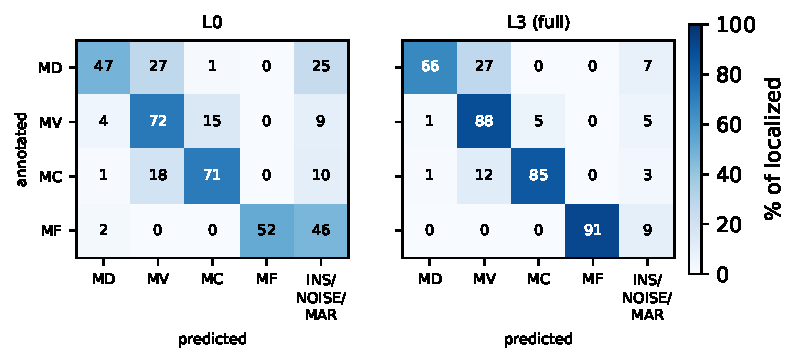
\includegraphics[width=0.55\linewidth]{figs/rq1_confusion.pdf}
\caption{RQ1, TEST: confusion among localized target instances for L0 (left) and L3 (right), seeds 0--2 pooled; each row is a percentage of localized instances of the annotated class (missed instances excluded; right block: predicted INS, NOISE or MAR).}
\label{fig:rq1_confusion}
\end{figure}

\paragraph{Scope.}
Size and composition vary together, so the comparisons give combined effects. L0 has 103 images; DS-ORG is about 42\% of L2+ORG, and L2+ORG and L3 are alternative extensions of L2, so their difference does not isolate copy-paste. One fixed TEST split and three seeds; the crowded (7) and INS-only (6) subsets are descriptive.


\subsection{RQ2 on DS-F2\_v9.0.5: Cascade, Oracle and the Identification Ceiling}
\label{sec:exp:rq2v9}


\paragraph{Setup.} VAL selected \texttt{best.pt}, so VAL numbers are not held out and serve only as a consistency check. Metrics are macro-F1 over the four species at score$\ge$0.25 and IoU$\ge$0.5. Stage~2 is a ConvNeXt-T~\cite{liu2022convnext} (CE or part-aware head), DINOv2, DINOv3 or BioCLIP~2, all fully fine-tuned. Detectors: E0 (three seeds), YOLO26l (one seed), RT-DETR-l~\cite{zhao2024rtdetr} (three seeds). Intervals are 95\% BCa bootstrap over test images (10{,}000 resamples, paired with the detector-only run) with a sign-flip permutation test~\cite{du2025pairedbootstrap}.

\paragraph{The cascade does not improve on the detector.} On TEST, E0 alone reaches 79.5\% macro-F1 and every one of the five stage-2 backbones lowers it: $\Delta$F1 is $-2.7$ [$-4.8$, $-0.3$] pp for ConvNeXt-T CE ($p_{\text{perm}}=0.013$), $-1.4$ [$-3.7$, $+1.3$] for parts, $-1.7$ [$-3.5$, $+0.1$] for DINOv2, $-2.0$ [$-4.0$, $+0.3$] for DINOv3 and $-1.1$ [$-2.7$, $+0.8$] for BioCLIP~2 (E0, nine pairs). With YOLO26l (80.5\%) the shifts are $-2.1$ to $-4.0$ pp, and with RT-DETR-l (74.6\%) $-2.3$ to $-5.1$ pp. Single-configuration intervals often include zero (73 images), but the sign is the same in all 5$\times$3 configurations (YOLO26l has one seed); McNemar $p$ varies between seeds ($0.005$--$0.51$ for CE with E0), so we do not summarize it.

\paragraph{Why: a ceiling at identification.} With ground-truth crops the classifiers reach 82.7--83.8\% species accuracy on TEST (87--88\% on VAL), regardless of backbone family; a better backbone does not lift the ceiling. This is a plateau, not a proven information limit: the detector alone is at $\approx$84\% among localized objects (82.2/97.7). Across the 15 classifiers, 60.0\% of instances are correct for all and 4.9\% are wrong for all; majority vote gives 86.3\% against a mean of 83.4\%. Errors are confident (69.4\% have max-softmax $\ge0.8$) and concentrated in the MD/MV/MC family (family-level accuracy 96.0\% vs.\ 80.6\% by species). Abstention (keeping the detector label below a confidence $\tau$) gains at most $+0.2$\,pp. Confident learning flags 3.7\% (127/3{,}470) of the TEST crops and 4.1\% of VAL as suspect labels, mostly NOISE$\leftrightarrow$MF, MD$\leftrightarrow$MV and MC$\leftrightarrow$MV; we have no expert review, so ``suspect'' does not mean ``wrong''. The rate is in the range reported for curated benchmarks~\cite{northcutt2021pervasive}.

\paragraph{Limitations and open items.} No expert re-labelled the confusable pairs, so ambiguity cannot be separated from label noise. A near-duplicate check finds no VAL or TEST image with thumbnail similarity $\ge0.98$ to a training image, but 4.7\% of TEST crops reach it against some training crop (plausibly glue background), so we do not claim absence of leakage at crop level. \paragraph{Background class.} A natural fix for the species that the seven-way head sends to \emph{non-species} is an eight-way head with an explicit background class trained on detector false positives (BG). With three classifier seeds on the E0 detectors, BG gives $\Delta$F1 $-2.8$ [$-4.8$, $-0.4$] pp on TEST ($p_{\text{perm}}=0.010$) and $-5.4$ pp on VAL, the same as the CE control ($-2.7$ and $-5.5$ pp); its accuracy on ground-truth crops is $77.6\pm2.8$\% (TEST), not higher. The background class does not remove the loss. Oracle accuracy with 25\%, 50\% and 100\% of the training crops (ConvNeXt-T, one seed) is flat on TEST (83.0, 81.7, 82.6\%), compatible with ambiguity but not proof of it.

\begin{table}[t]
\centering
\caption{Per-species TEST results, E0 alone vs.\ the ConvNeXt-T CE cascade (mean of nine pairs; recall, precision and F1 in \%; count error = mean $|n_{\text{pred}}-n_{\text{GT}}|$ per image).}
\label{tab:persp}
\footnotesize
\setlength{\tabcolsep}{3pt}
\begin{tabular}{@{}lrrrrrrrr@{}}
\toprule
 & \multicolumn{4}{c}{E0 alone} & \multicolumn{4}{c}{Cascade} \\
\cmidrule(r){2-5}\cmidrule(l){6-9}
 & R & P & F1 & err & R & P & F1 & err \\
\midrule
MD & 64.9 & 78.8 & 71.2 & 1.17 & 61.4 & 70.4 & 65.5 & 1.49 \\
MV & 87.9 & 69.0 & 77.3 & 1.67 & 85.6 & 68.8 & 76.2 & 1.96 \\
MC & 84.6 & 86.1 & 85.3 & 0.76 & 84.3 & 86.3 & 85.3 & 0.78 \\
MF & 86.0 & 82.9 & 84.4 & 0.83 & 87.1 & 74.9 & 80.5 & 1.41 \\
\bottomrule
\end{tabular}
\end{table}

\paragraph{Fusion, margin, cost and localization.} The detector exposes only its top-1 class and score, so a fusion with its full class distribution was not run. On TEST, F1 (nine pairs) is 79.5\% for E0, 76.9\% for the cascade and 79.6\% for a soft fusion, which only matches the detector. Two variants of the ConvNeXt-T CE cascade (species accuracy on TEST, H100) do not change the picture: relabelling only the proposals called a species gives $-1.5$ [$-3.2$, $+0.3$] pp against the detector alone, and a late fusion with its top-1 score (weight chosen on VAL) $+0.3$ [$-0.1$, $+0.7$] pp; on the B200 the same fusion gave $+1.3$ pp, so we read it as hardware-dependent noise. Retraining the classifier with a smaller context margin makes the cascade worse: $-0.9$ pp at 75\% of the box per side (paper setting), $-2.8$ [$-5.0$, $-0.3$] at 25\% and $-2.5$ [$-5.3$, $+0.6$] at 0\%. These runs use another GPU than the main table (detector alone differs by 0.6 pp), so margins are compared only among themselves. E0 localizes $97.7\pm0.4$\% of the TEST species instances (RT-DETR 98.5\%), so the remaining error is identification.

\subsection{RQ3: Transfer of Tiny-Object Methods}
\label{sec:exp:rq3}

\paragraph{Protocol.}
RQ3 was run as a separate campaign on a different GPU (L40S) with the same recipe as E0 (YOLO26m, 150 epochs, batch 8, \texttt{imgsz} 1920, patience 30) and the same data, so its own E0 (three seeds) is the only control for the variants below; we do not mix it with the E0 of other tables. The variants are: NWD ($w{=}0.5$, $C{=}44$\,px) in the loss only, NWD in the assigner only, NWD plus RFLA, the scale-adaptive GCD ($w{=}0.5$), Wise-IoU v3, a P2 head, training and inference at \texttt{imgsz} 2560 (batch 4), and, with one seed, YOLO11m. The metric is species accuracy on TEST: a ground-truth species instance counts as correct if a detection with score $\ge0.25$ matches it at IoU$\ge$0.5 and has the right class (equal to micro recall over the 1{,}210 species instances). $\Delta$ is the per-seed difference to E0 of the same seed, with a 95\% bootstrap interval over images (10{,}000 resamples), and $p$ is Holm-corrected over the eight comparisons.

\paragraph{No variant improves on E0.}
Table~\ref{tab:rq3_main} shows that no variant has a positive $\Delta$ whose interval excludes zero. GCD, Wise-IoU v3 and NWD in the assigner only are indistinguishable from E0 ($\Delta$ between $-0.3$ and $+0.3$\,pp); their intervals are $\approx\pm1.7$\,pp wide, so we claim no difference detected, not equivalence. P2, \texttt{imgsz} 2560 and NWD in the loss only are $2.5$--$3.8$\,pp below E0 and do not survive the Holm correction ($p=0.14$, 0.057, 0.084). Only NWD+RFLA is $8.8$\,pp below E0 (Holm $p=0.002$) and unstable: one seed stopped early at epoch~40 with its best epoch near~10, and another diverged (classification loss in the thousands from epoch~27, \texttt{nan} at epoch~30); we kept the recipe and did not retry, so the mean of $72.9\pm7.5$\% includes both. NWD acts through its loss, not through the assigner: the assigner-only variant equals E0 while the loss-only variant is $2.5$\,pp lower. YOLO11m (one seed, exploratory) is $1.2$\,pp below, interval including zero.

\begin{table}[t]
\centering
\caption{RQ3 on TEST (73 images, 1{,}210 species instances), YOLO26m, L40S campaign; three seeds unless noted. Accuracy: mean$\pm$std. $\Delta$: paired difference to E0 of the same seed in pp, with 95\% bootstrap interval over images; $p$: Holm over the eight three-seed variants (YOLO11m, one seed, is outside the family; its $p$ is not corrected). Recall (\%) by object size $\sqrt{wh}$ ($n=613$, 376, 221). VAL selected \texttt{best.pt} and is not held out; all numbers are TEST.}
\label{tab:rq3_main}
\footnotesize
\setlength{\tabcolsep}{2.5pt}
\resizebox{\linewidth}{!}{%
\begin{tabular}{@{}lrrrrrr@{}}
\toprule
 & Acc. (\%) & $\Delta$ [95\% CI] & $p$ & $<$32 & 32--48 & $\ge$48 \\
\midrule
E0 (CIoU) & 81.7$\pm$1.2 & --- & --- & 79.4 & 81.0 & 89.4 \\
GCD & 81.5$\pm$0.4 & $-0.2$ [$-1.8$, $+1.6$] & 1.00 & 78.3 & 80.5 & 92.3 \\
Wise-IoU v3 & 81.4$\pm$1.0 & $-0.3$ [$-1.9$, $+1.5$] & 1.00 & 78.9 & 79.6 & 91.4 \\
NWD, assigner only & 82.0$\pm$1.9 & $+0.3$ [$-1.4$, $+2.4$] & 1.00 & 79.4 & 80.6 & 91.7 \\
NWD, loss only & 79.3$\pm$3.4 & $-2.5$ [$-4.5$, $-0.5$] & 0.084 & 74.0 & 80.8 & 91.3 \\
P2 head & 79.0$\pm$2.7 & $-2.8$ [$-5.0$, $-0.4$] & 0.14 & 74.0 & 80.1 & 91.0 \\
\texttt{imgsz} 2560 & 78.0$\pm$3.3 & $-3.8$ [$-6.1$, $-1.1$] & 0.057 & 72.8 & 79.3 & 90.0 \\
NWD + RFLA & 72.9$\pm$7.5 & $\mathbf{-8.8}$ [$-12.7$, $-4.9$] & 0.002 & 63.3 & 78.5 & 90.0 \\
\midrule
YOLO11m (1 seed) & 81.0 & $-1.2$ [$-4.4$, $+2.1$] & --- & 76.3 & 83.0 & 90.5 \\
\bottomrule
\end{tabular}%
}
\end{table}

\paragraph{Tuned NWD against a same-GPU control.}
We also trained NWD (loss and assigner) with other constants on the H100, with its own E0 control (three seeds, $82.2\pm1.9$\%). $w{=}0.5$, $C{=}22$\,px gives $81.7\pm1.5$\% ($-0.5$ [$-2.7$, $+1.8$] pp); $w{=}1.0$, $C{=}44$\,px collapses to $53.9\pm1.3$\% ($-28.3$ [$-34.9$, $-21.4$] pp); $w{=}0.5$, $C{=}88$\,px, with two seeds, gives $81.8\pm3.7$\% ($-0.7$ [$-3.0$, $+1.8$] pp; seeds $-5.2$, $+3.8$). None beats the control.

\paragraph{Recall by object size.}
The smallest objects do not benefit from any variant: the recall below 32\,px is at most equal to E0 (E0 79.4\%, NWD assigner-only 79.4\%) and lower for all others, down to 63.3\% for NWD+RFLA (Table~\ref{tab:rq3_main}). The gains above 48\,px (0.6 to 2.9\,pp) come with a seed spread of 1--5\,pp and are not statistically supported. This agrees with the localization result of RQ2: E0 localizes $97.7\pm0.4$\% of the species instances, so a box-similarity loss has little to repair and the smallest objects are limited by identification.

\paragraph{Sliced inference, test-time augmentation and ensembling.}
We apply three inference-time methods to the three E0 detectors (mAP@50 under a confidence-0.0 evaluator, not the species harness; WBF is a single result over the three seeds). Sliced inference (512\,px tiles, 25\% overlap) reaches a species recall of $86.7\pm1.8$\% and mAP@50 $69.5\pm0.8$, against $35.5\pm0.9$\% and $9.5\pm1.0$ for the same detector run on the whole frame resized to 512\,px. That comparison is unfair (the resize shrinks the frame $\approx$3.75$\times$); the relevant baseline is E0 at native resolution (mAP@50 $84.2\pm0.5$, mAP@50:95 $61.7\pm0.1$), and slicing a detector trained at 1920\,px with 512\,px tiles does not reach it. TTA at 1920 adds $+0.4$ mAP@50 and $+0.5$ mAP@50:95, a small gain. A weighted-boxes-fusion ensemble of the three E0 detectors gives mAP@50 $83.6$, below the single-model mean (84.2), so we find no gain from ensembling either.


\paragraph{Why the aerial loss recipes do not transfer here.}
Three properties of our regime differ from the benchmarks on which NWD, RFLA and SAHI were validated. First, the objects are tiny by the COCO convention but the images are processed at native resolution: a 44-px fly spans about five cells of the stride-8 feature map, whereas the AI-TOD regime for which NWD was designed has objects of a few pixels after the network's own downscaling; the IoU sensitivity that NWD corrects is therefore much milder. Second, YOLO26 already uses a task-aligned dynamic assignment and an NMS-free one-to-one head~\cite{yolo26}; the reported gains of NWD and RFLA come from anchor-based or two-stage detectors with static IoU-threshold assignment~\cite{wang2021nwd,xu2022rfla,xu2022aitod}, where a Gaussian similarity changes which anchors become positive. Third, sliced inference is designed for the case where the alternative is to downscale a large image below the object scale~\cite{akyon2022sahi}; here the detector already runs at native scale. These are untested explanations; $C=44$\,px was measured on an earlier data version.

\subsection{Error Analysis}
\label{sec:exp:errors}

Confusion rates among TEST species for E0 and the E0\,+\,CE cascade (nine detector--classifier pairs, mean; $\Delta$ is mean$\pm$std of the paired difference; MV$\to$non-species 4.7\% to 1.5\%, MC$\to$non-species 3.0\% to 0.7\%). The dominant error of the detector is MD$\rightarrow$MV (26.3\%) and MC$\rightarrow$MV (11.7\%). The cascade moves these only partly: MD$\rightarrow$MV falls by $5.3\pm3.5$\,pp, but the instances do not become correct; MD$\rightarrow$\emph{non-species} rises by $8.0\pm5.1$\,pp (7.0\% to 15.0\%) and MV$\rightarrow$MD rises by $4.9\pm1.2$\,pp (1.4\% to 6.3\%). The seven-way head therefore trades one error for others: MD ends at 61.4\% correct against 64.9\% for the detector. MC$\rightarrow$MV does not move ($+1.4\pm6.2$\,pp). MF is never confused with another species by either system; its errors are non-species and missed objects, which the cascade cannot repair because it does not change boxes (Table~\ref{tab:persp}: recall 86.0\% vs.\ 87.1\%, but precision falls from 82.9\% to 74.9\% as other species are relabelled MF). 




\section{\uppercase{Conclusions}}
\label{sec:conclusion}

We asked what limits species-level reading of sticky traps and which lever moves that limit. Along a ladder of five cumulative training sets, species accuracy rises from 56.1\% to 82.2\%, with the largest gains on objects below 32\,px and insect-only plates and part of the look-alike confusion shrinking; but random subsamples of the final training set of the size of L1 and L2 reach the same accuracy, so from L1 to L2 the rise is mostly the number of images, not targeting, but not the L0 deficit (a random 103-image subsample is 19\,pp better). Identification did not move with the classifier: with our recipe, a detect-then-classify cascade does not improve on the single-stage detector in any of 15 configurations (nor with species-only relabelling, late fusion or other crop margins), ground-truth-crop accuracy saturates near 83\% for five classifiers (four backbones), and the residual errors are mostly confident and concentrated in MD/MV/MC (only 4.9\% are wrong for all fifteen classifiers), so this is a plateau, not a proven information limit; label noise or the crop recipe cannot be excluded. Tiny-object methods from aerial imagery bring no gain detectable here: none of eight variants improves species accuracy over a same-campaign control with three seeds (all differences between $-3.8$ and $+0.3$\,pp except NWD with RFLA at $-8.8$\,pp), and none raises the recall of objects below 32\,px. For practitioners of trap-based monitoring, our results suggest that, among the levers tested, more annotated plates helped most (whether targeting adds beyond quantity remains open), and that investigating the remaining confusion within the housefly/blowfly/flesh-fly family as a possible labeling and imaging problem, which expert re-annotation could settle.

\paragraph{Limitations.} One facility and one test split (73 images; 7 crowded and 6 insect-only plates), whose 95\% intervals are about $\pm2$\,pp wide, so effects smaller than that cannot be resolved; three seeds; the cascade experiments use the final dataset only. Cross-trap-colour evaluation~\cite{ong2025} was not done; the split rule by plate is not documented, so leakage between images of the same plate cannot be excluded; RQ3 and part of the equal-size runs used a different GPU than RQ1/RQ2; checkpoints were selected on VAL, so no never-consulted hold-out exists. The tiny-object variants were tuned only for NWD (three settings, one with a single seed), so this is ``no gain detected here'', not proof of none; the NWD+RFLA drop stems from unstable seeds. Generalization beyond this facility is untested and the code and configurations will be released but the images will not, so the ladder cannot be reproduced independently.

\paragraph{Future work.} Out-of-distribution rejection for novel species~\cite{opensect2025}, expert re-annotation of the confusable pairs, a size control that separates label quality from quantity at the earliest lot, edge deployment.


\section*{\uppercase{Acknowledgements}}

Anonymous during review.

\bibliographystyle{apalike}
{\small
\bibliography{main}}

\end{document}
